% Isolated Clusters: Integration into full AMC40 Firmware
% Author:	Dónal Murray
% Date:		30 Mar 2017

% --PREAMBLE--
\documentclass[10pt,a4paper,twoside]{article}
\usepackage[margin=2.54cm]{geometry} % 2.54cm margins
\usepackage{graphicx} % images
\usepackage{tikz}

\usetikzlibrary{positioning,fit,calc}
\tikzstyle{block} = [draw, rectangle, minimum height=3em, minimum width=7em]
\tikzstyle{fifo} = [draw, rectangle, minimum height=8em, minimum width=7em]
\tikzstyle{bigblock} = [draw, rectangle, minimum height=8em, minimum width=10em]

% --BODY--
\begin{document}
\begin{figure}
	\centering\section*{Isolated cluster flagging module: position in AMC40 Firmware}

	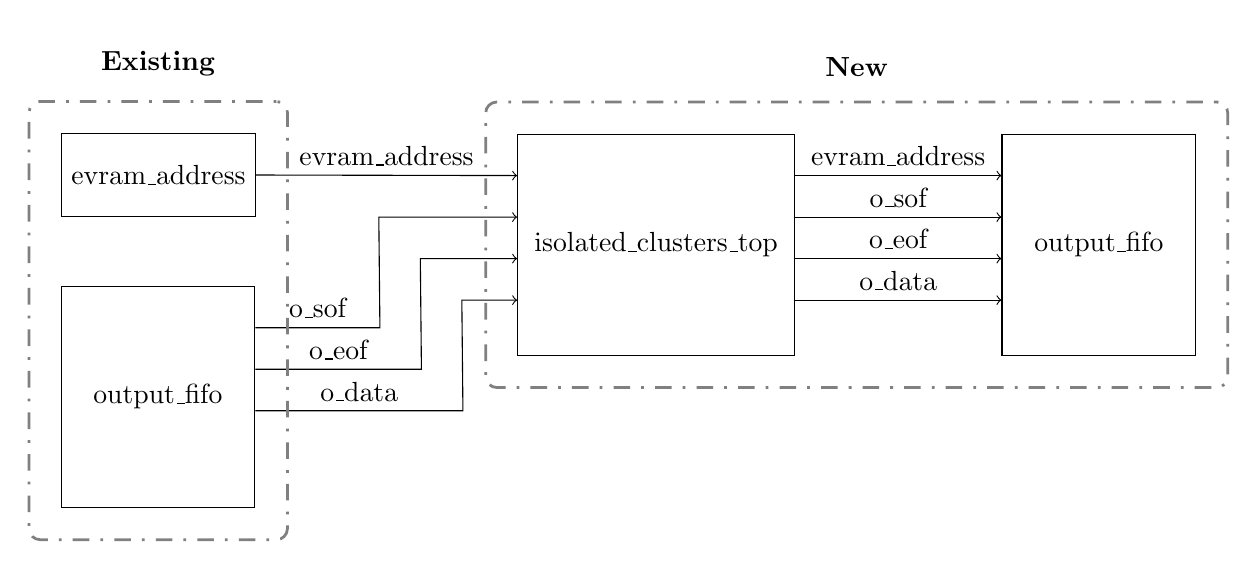
\begin{tikzpicture}[auto]
		% anchor block
		\node[coordinate] (anchor) {};
		\node[coordinate,right= 18em of anchor] (anchormid) {};
		\node[coordinate,right= 16em of anchormid] (anchorright) {};

		% evram
		\node[block,right= -3.5em of anchor] (evram) {evram\_address};

		% fifo 0
		\node[fifo,below= 4em of anchor] (fifo0) {output\_fifo};
		\node[coordinate,above= 2.5em of fifo0.east] (fifo0pin0) {};
		\node[coordinate,below= 1.5em of fifo0pin0] (fifo0pin1) {};
		\node[coordinate,below= 1.5em of fifo0pin1] (fifo0pin2) {};
		\node[coordinate,below= 1.5em of fifo0pin2] (fifo0pin3) {};

		% isolated clusters
		\node[bigblock,below= -1.5em of anchormid] (clust) {isolated\_clusters\_top};
		\node[coordinate,above= 2.5em of clust.west] (clustpin0) {};
		\node[coordinate,below= 1.5em of clustpin0] (clustpin1) {};
		\node[coordinate,below= 1.5em of clustpin1] (clustpin2) {};
		\node[coordinate,below= 1.5em of clustpin2] (clustpin3) {};
		\node[coordinate,above= 2.5em of clust.east] (clustpin4) {};
		\node[coordinate,below= 1.5em of clustpin4] (clustpin5) {};
		\node[coordinate,below= 1.5em of clustpin5] (clustpin6) {};
		\node[coordinate,below= 1.5em of clustpin6] (clustpin7) {};

		% fifo 1
		\node[fifo,below= -1.5em of anchorright] (fifo1) {output\_fifo};
		\node[coordinate,above= 2.5em of fifo1.west] (fifo1pin0) {};
		\node[coordinate,below= 1.5em of fifo1pin0] (fifo1pin1) {};
		\node[coordinate,below= 1.5em of fifo1pin1] (fifo1pin2) {};
		\node[coordinate,below= 1.5em of fifo1pin2] (fifo1pin3) {};

		% join evram to clust
		\draw [->] (evram.east) -- node{evram\_address} (clustpin0);

		% join fifo0 to clust
		\node[coordinate,right= 4.5em of fifo0pin0] (fcmid0b) {};
		\node[coordinate,left= 5em of clustpin1] (fcmid0t) {};
		\node[coordinate,right= 6em of fifo0pin1] (fcmid1b) {};
		\node[coordinate,left= 3.5em of clustpin2] (fcmid1t) {};
		\node[coordinate,right= 7.5em of fifo0pin2] (fcmid2b) {};
		\node[coordinate,left= 2em of clustpin3] (fcmid2t) {};
		\draw [->] (fifo0pin0) -- node{o\_sof} (fcmid0b) -- (fcmid0t) -- (clustpin1);
		\draw [->] (fifo0pin1) -- node{o\_eof} (fcmid1b) -- (fcmid1t) -- (clustpin2);
		\draw [->] (fifo0pin2) -- node{o\_data} (fcmid2b) -- (fcmid2t) -- (clustpin3);

		% join clust to fifo1
		\draw [->] (clustpin4) -- node{evram\_address} (fifo1pin0);
		\draw [->] (clustpin5) -- node{o\_sof} (fifo1pin1);
		\draw [->] (clustpin6) -- node{o\_eof} (fifo1pin2);
		\draw [->] (clustpin7) -- node{o\_data} (fifo1pin3);

		% define the boxes
  		\tikzset{blue dotted/.style={draw=black!50!white, line width=1pt,
                               dash pattern=on 1pt off 4pt on 6pt off 4pt,
                                inner sep=4mm, rectangle, rounded corners}};

  		% draw the boxes
  		\node (first dotted box) [blue dotted, fit = (evram) (fifo0)] {};
  		\node (second dotted box) [blue dotted, fit = (clust) (fifo1)] {};
  		% label the boxes
  		\node at (first dotted box.north) [above, inner sep=3mm] {\textbf{Existing}};
  		\node at (second dotted box.north) [above, inner sep=3mm] {\textbf{New}};
	\end{tikzpicture}
	\caption{Block diagram showing the position of the new block}
\end{figure}

\begin{figure}
	\centering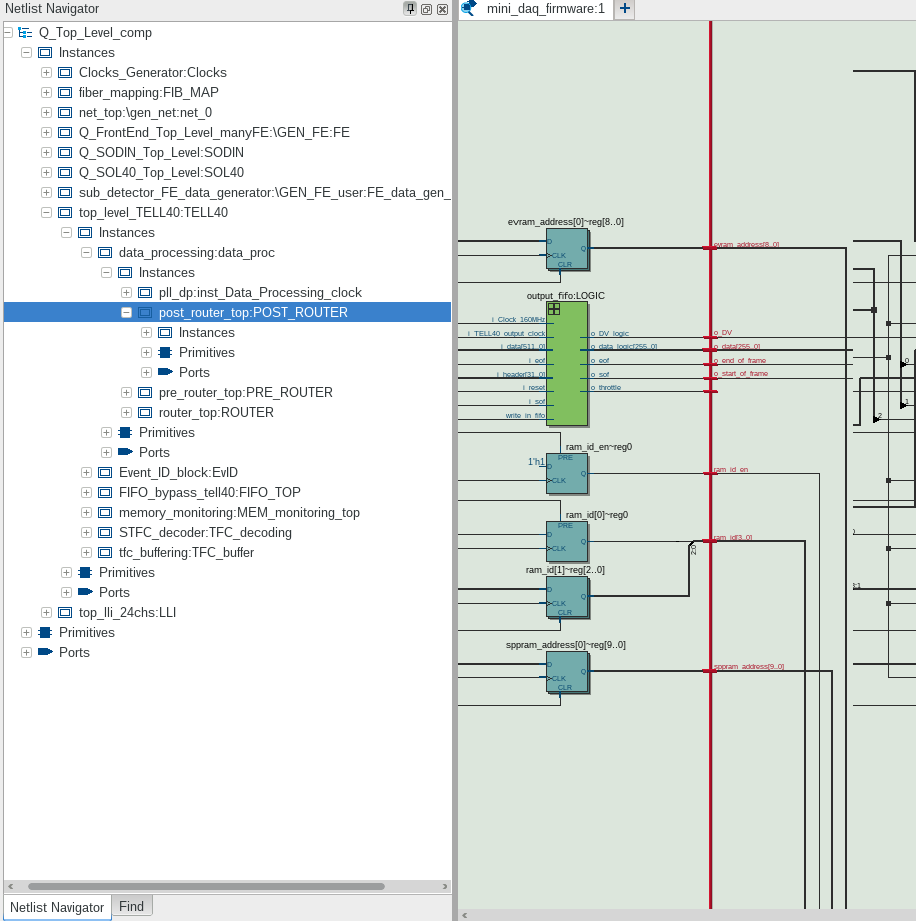
\includegraphics[trim={0 10cm 3cm 0},clip,scale=0.5]{img/postrouterOut}
	\caption{A screenshot of the position of the isolated clusters block in amc40firmware (RTL view)}
\end{figure}
\end{document}
